\section{Algoritmul de extragere a informației}

Înțelegerea conținutului bonurilor fiscale din imagini reprezintă principala provocare a acestui proiect și funcționalitatea în jurul căreia este construită întreaga aplicație. În mod natural, aceasta se desparte în două sarcini:

\begin{itemize}
  \item 
  Recunoașterea textului;
  \item
  Extragerea informațiilor din textul neprocesat;
\end{itemize}

Metode mai bune pentru a rezolva această provocare pot ține cont de imagini și pentru a doua sarcină și pot folosi metode mai avansate, de \emph{machine learning}, pe măsură ce sunt colectate mai multe date. Aceste opțiuni sunt subiectul unor cercetări viitoare.

\subsection{Recunoașterea textului}

O constrângere pentru rezolvarea acestei sarcini este aceea ca procesarea să se facă pe dispozitiv. Astfel, datele utilizatorului nu părăsesc dispozitivul decât cu acordul său.

O soluție \emph{open source} populară pentru rezolvarea problemelor OCR este \emph{Tesseract} \cite{Tesseract}. Pentru dezvoltatorii de aplicații mobile, Google oferă librăria \emph{Firebase Vision}, cu suport gratuit pentru OCR pe dispozitiv. Comparația dintre cele două soluții a fost făcută astfel:

\begin{itemize}
  \item 
  Firebase Vision a fost rulat folosind un test de instrumentare, întrucât această librărie nu poate rula decât pe un dispozitiv mobil;
  \item
  Tesseract a fost rulat pe un computerul personal, folosind \emph{Python};
  \item
  Imaginea a fost pre-procesată doar pentru Tesseract, întrucât această librărie nu oferă o performanță satisfăcătoare pe imagini neprocesate;
  \item
  Preprocesarea a constat în aplicarea unui algoritm care să elimine fundalul, să transforme imaginea în alb-negru și să uniformizeze luminozitatea;
  \item
  Asupra ambelor rezultate a fost aplicat un algoritm care să grupeze chenarele de text pe linii;
  \item 
  Metrica după care au fost comparate cele două soluții este cea a acurateții textului recunoscut;
  \item 
  Cele două script-uri folosite pentru a rula cele două soluții se găsesc în anexa \ref{apx:Anexa1}.
\end{itemize}

În urma a mai multor teste, am observat că \emph{Tesseract} este mai susceptibil la zgomot și nu oferă rezultate de aceeași calitate ca \emph{Firebase Vision}. Un exemplu ușor este imaginea \ref{fig:exampleReceipt}. Textele extrase de cele două soluții sunt prezentate în figura \ref{fig:ocrResults}, unde se vede cantitatea de zgomot mai ridicată în rezultatul obținut cu \emph{Tesseract}. De asemenea, \emph{Tesseract} a emis alte câteva caractere non-utf8 de zgomot, ce nu au putut fi redate în acest text. De menționat este și efortul necesar pentru a integra \emph{Tesseract} într-o aplicație mobilă. În același timp, \emph{Firebase Vision} este disponibilă ca o dependință \emph{gradle}.

\begin{figure}[hb]
  \centering
  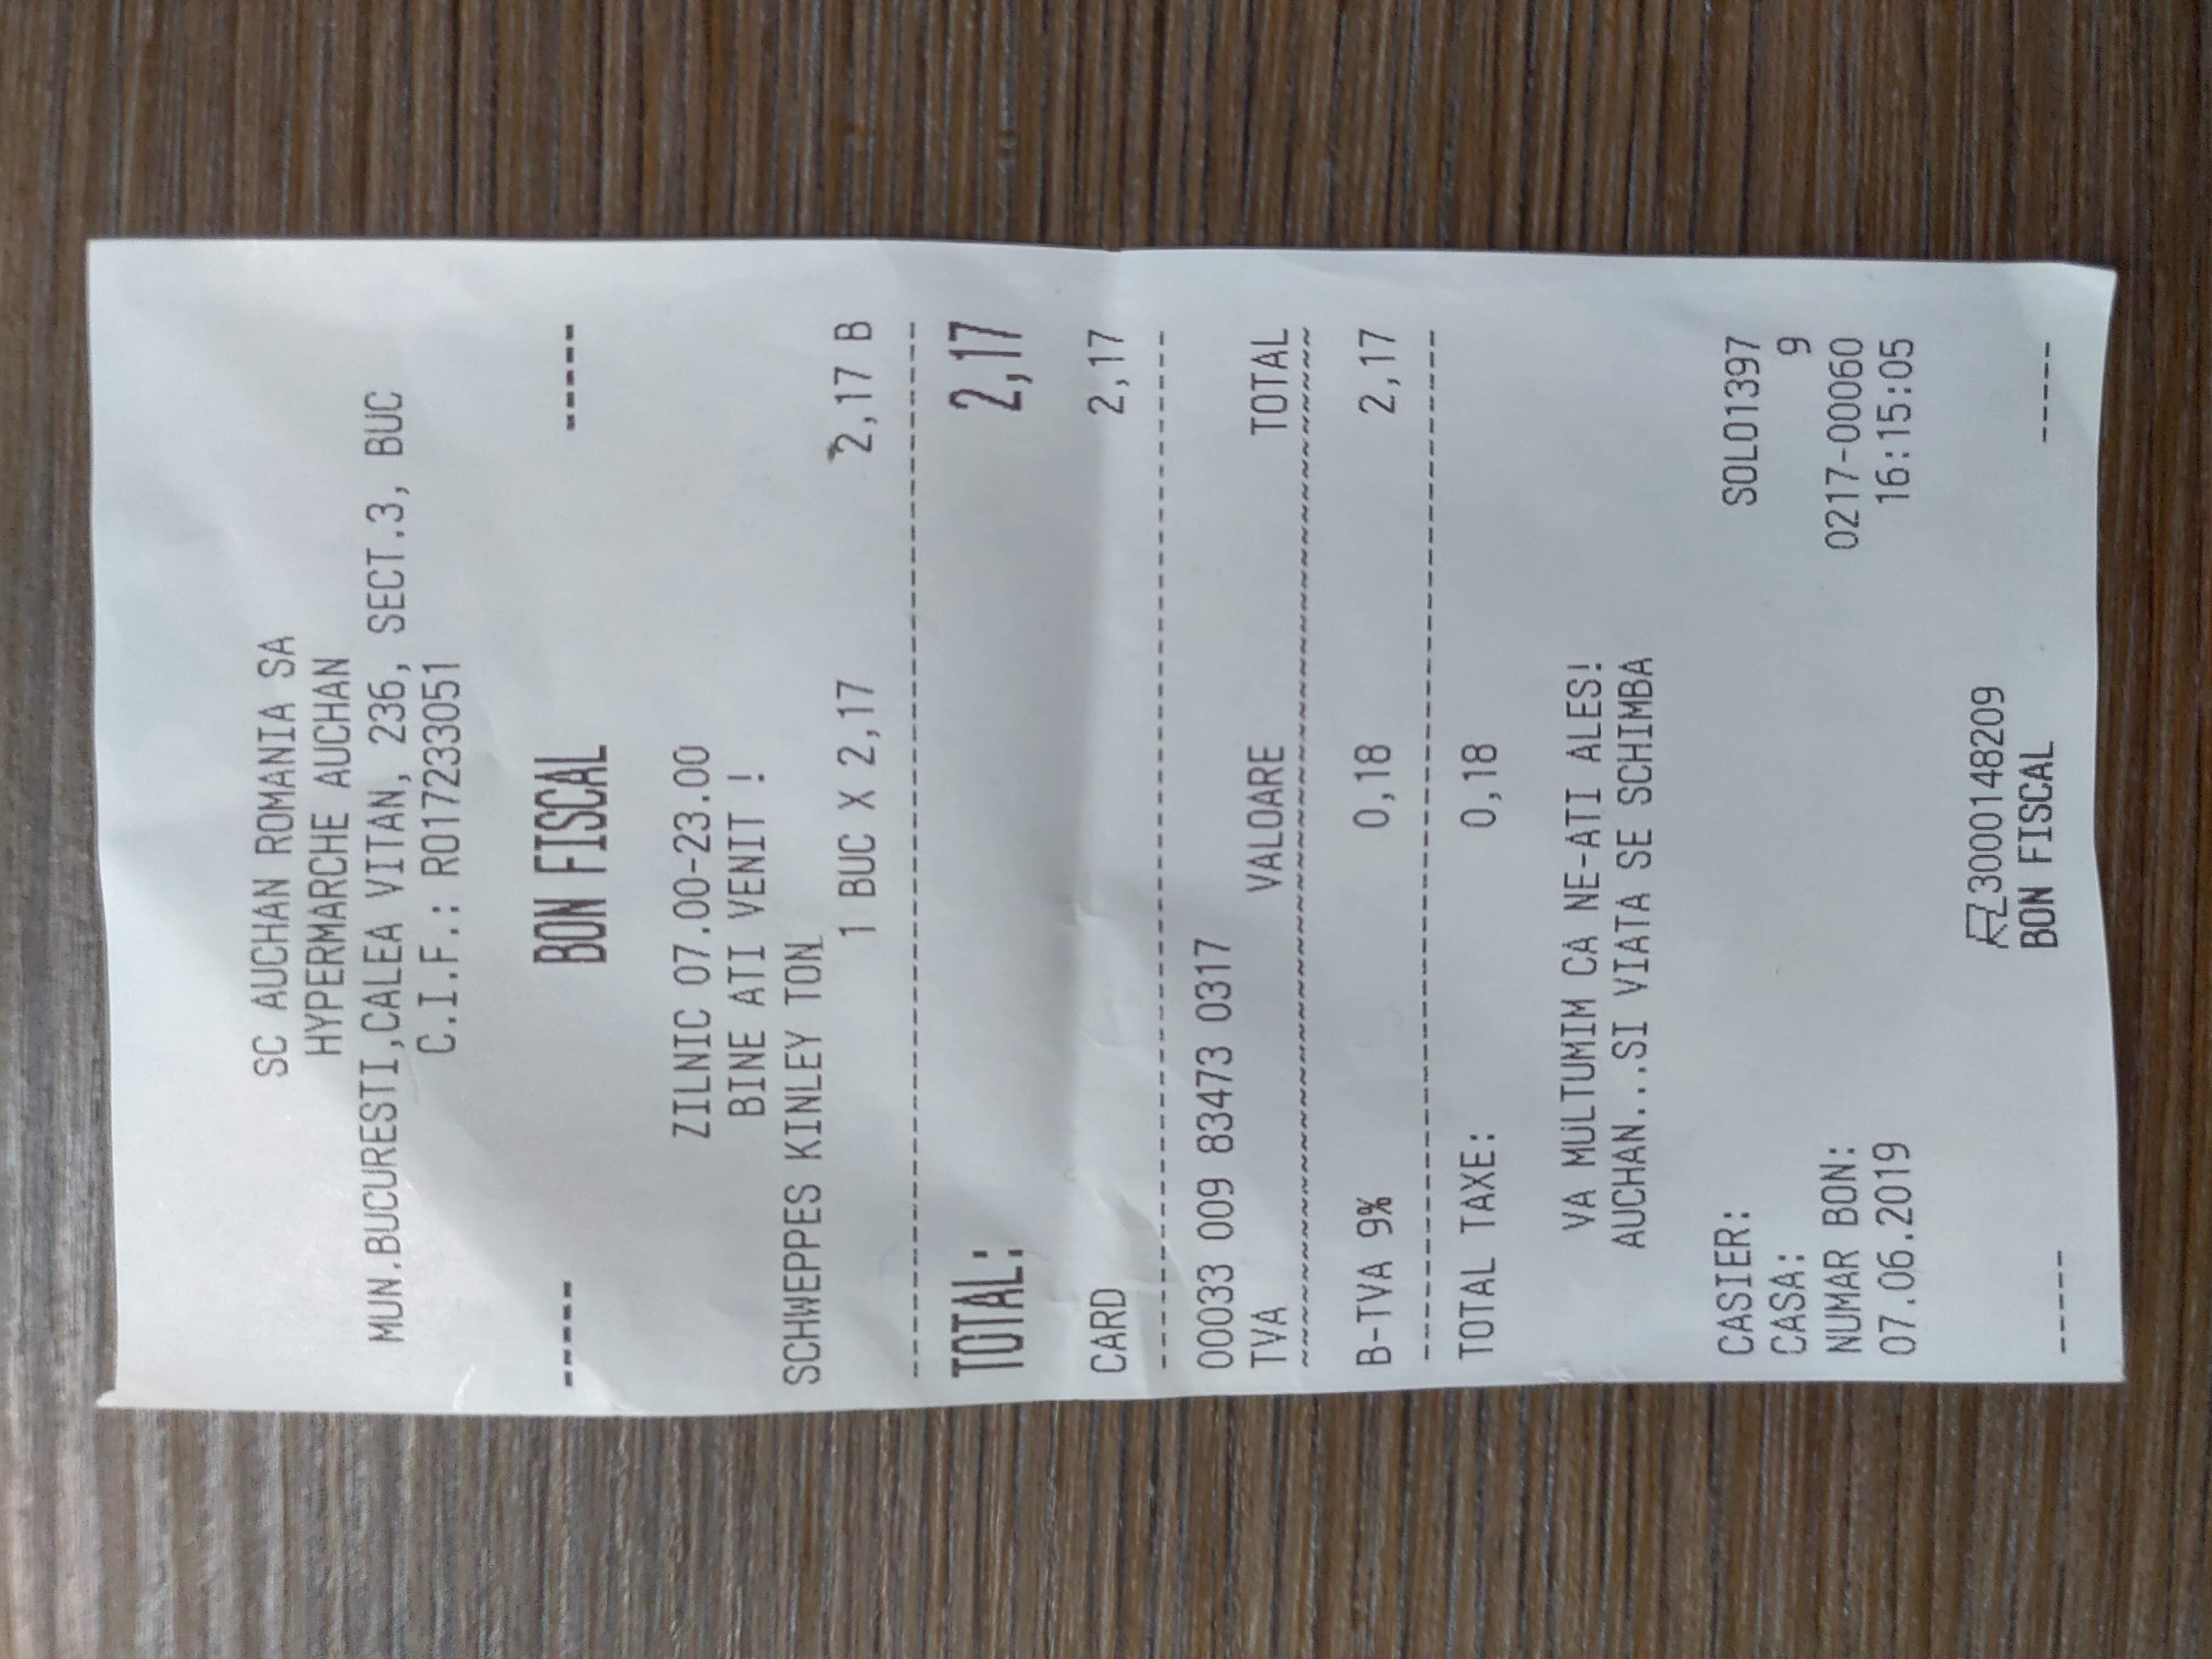
\includegraphics[width=0.5\textwidth,angle=-90]{receipt.jpg}
  \caption{Exemplu bon}
  \label{fig:exampleReceipt}
\end{figure}

\begin{figure}
  \begin{subfigure}{0.48\textwidth}
  \lstinputlisting[frame=single,breaklines=true,autogobble]{./samples/firebaseVisionOcrResult.txt}
  \caption{Firebase Vision OCR result}
  \label{fig:firebaseResult}
  \end{subfigure}
  \hfill
  \begin{subfigure}{0.48\textwidth}
  \lstinputlisting[frame=single,breaklines=true,autogobble]{./samples/tesseractOcrResult.txt}
  \caption{Tesseract OCR Result}
  \label{fig:tesseractResult}
  \end{subfigure}
  \caption{Textul extras de cele două soluții OCR}
  \label{fig:ocrResults}
\end{figure}

Performanța superioară a \emph{Firebase Vision} ar fi suficientă pentru a alege această librărie. La aceasta se adaugă și ușurința integrării și lipsa necesității de preprocesare. Dezavantajul major al acestei librării este integrarea unui serviciu extern, care nu este open source în codul aplicației, dar acesta nu este unul foarte mare pentru versiunea curentă a aplicației. Așadar, pentru sarcina de OCR am ales soluția \emph{Firebase Vision}.

\subsection{Extragerea informațiilor din text}

Procesarea textului rezultat în urma procesului de OCR se face pe baza unor reguli observate în majoritatea bonurilor fiscale. Firebase Vision returnează textul și chenarele de text, grupate în blocuri, linii și elemente, în funcție de coordonatele geometrice din imagine. Această organizare pe blocuri nu este de folos în procesarea de față, dar organizarea pe linii este, din moment ce informația din bonurile fiscale este așezată în format cheie-valoare, pe linii. De aceea, prima etapă în extragerea informațiilor este renunțarea la structura de blocuri și organizarea în linii raportate la întregul document. Această etapă se face după algoritmul:

\begin{enumerate}
  \item
  Extrage liniile din blocuri;
  \item
  Sortează liniile de sus în jos, în funcție de punctul lor de mijloc; Consideră liniile ca fiind elementele OCR;
  \item
  Grupează elementele OCR după distanța relativă dintre punctele lor de mijloc: elementele la o distanță mai mică de jumătate din media înălțimii tuturor elementelor se află în același grup;
\end{enumerate}

Implementarea acestui algoritm se găsește în Anexa \ref{apx:Anexa2}. Acest proces este ilustrat și în figura \ref{fig:ocrProcessing}. Organizarea la nivel de \textbf{bloc} este reprezentată în albastru, cea de \textbf{linie} în verde, iar cea de \textbf{element} în roșu. Se observă ca în organizarea dorită se renunță la structurile de blocuri, liniile se extind pe toată lățimea bonului, iar elementele devin fostele linii.

\begin{figure}[ht]
  \centering
  \begin{subfigure}{0.49\textwidth}
    \centering
    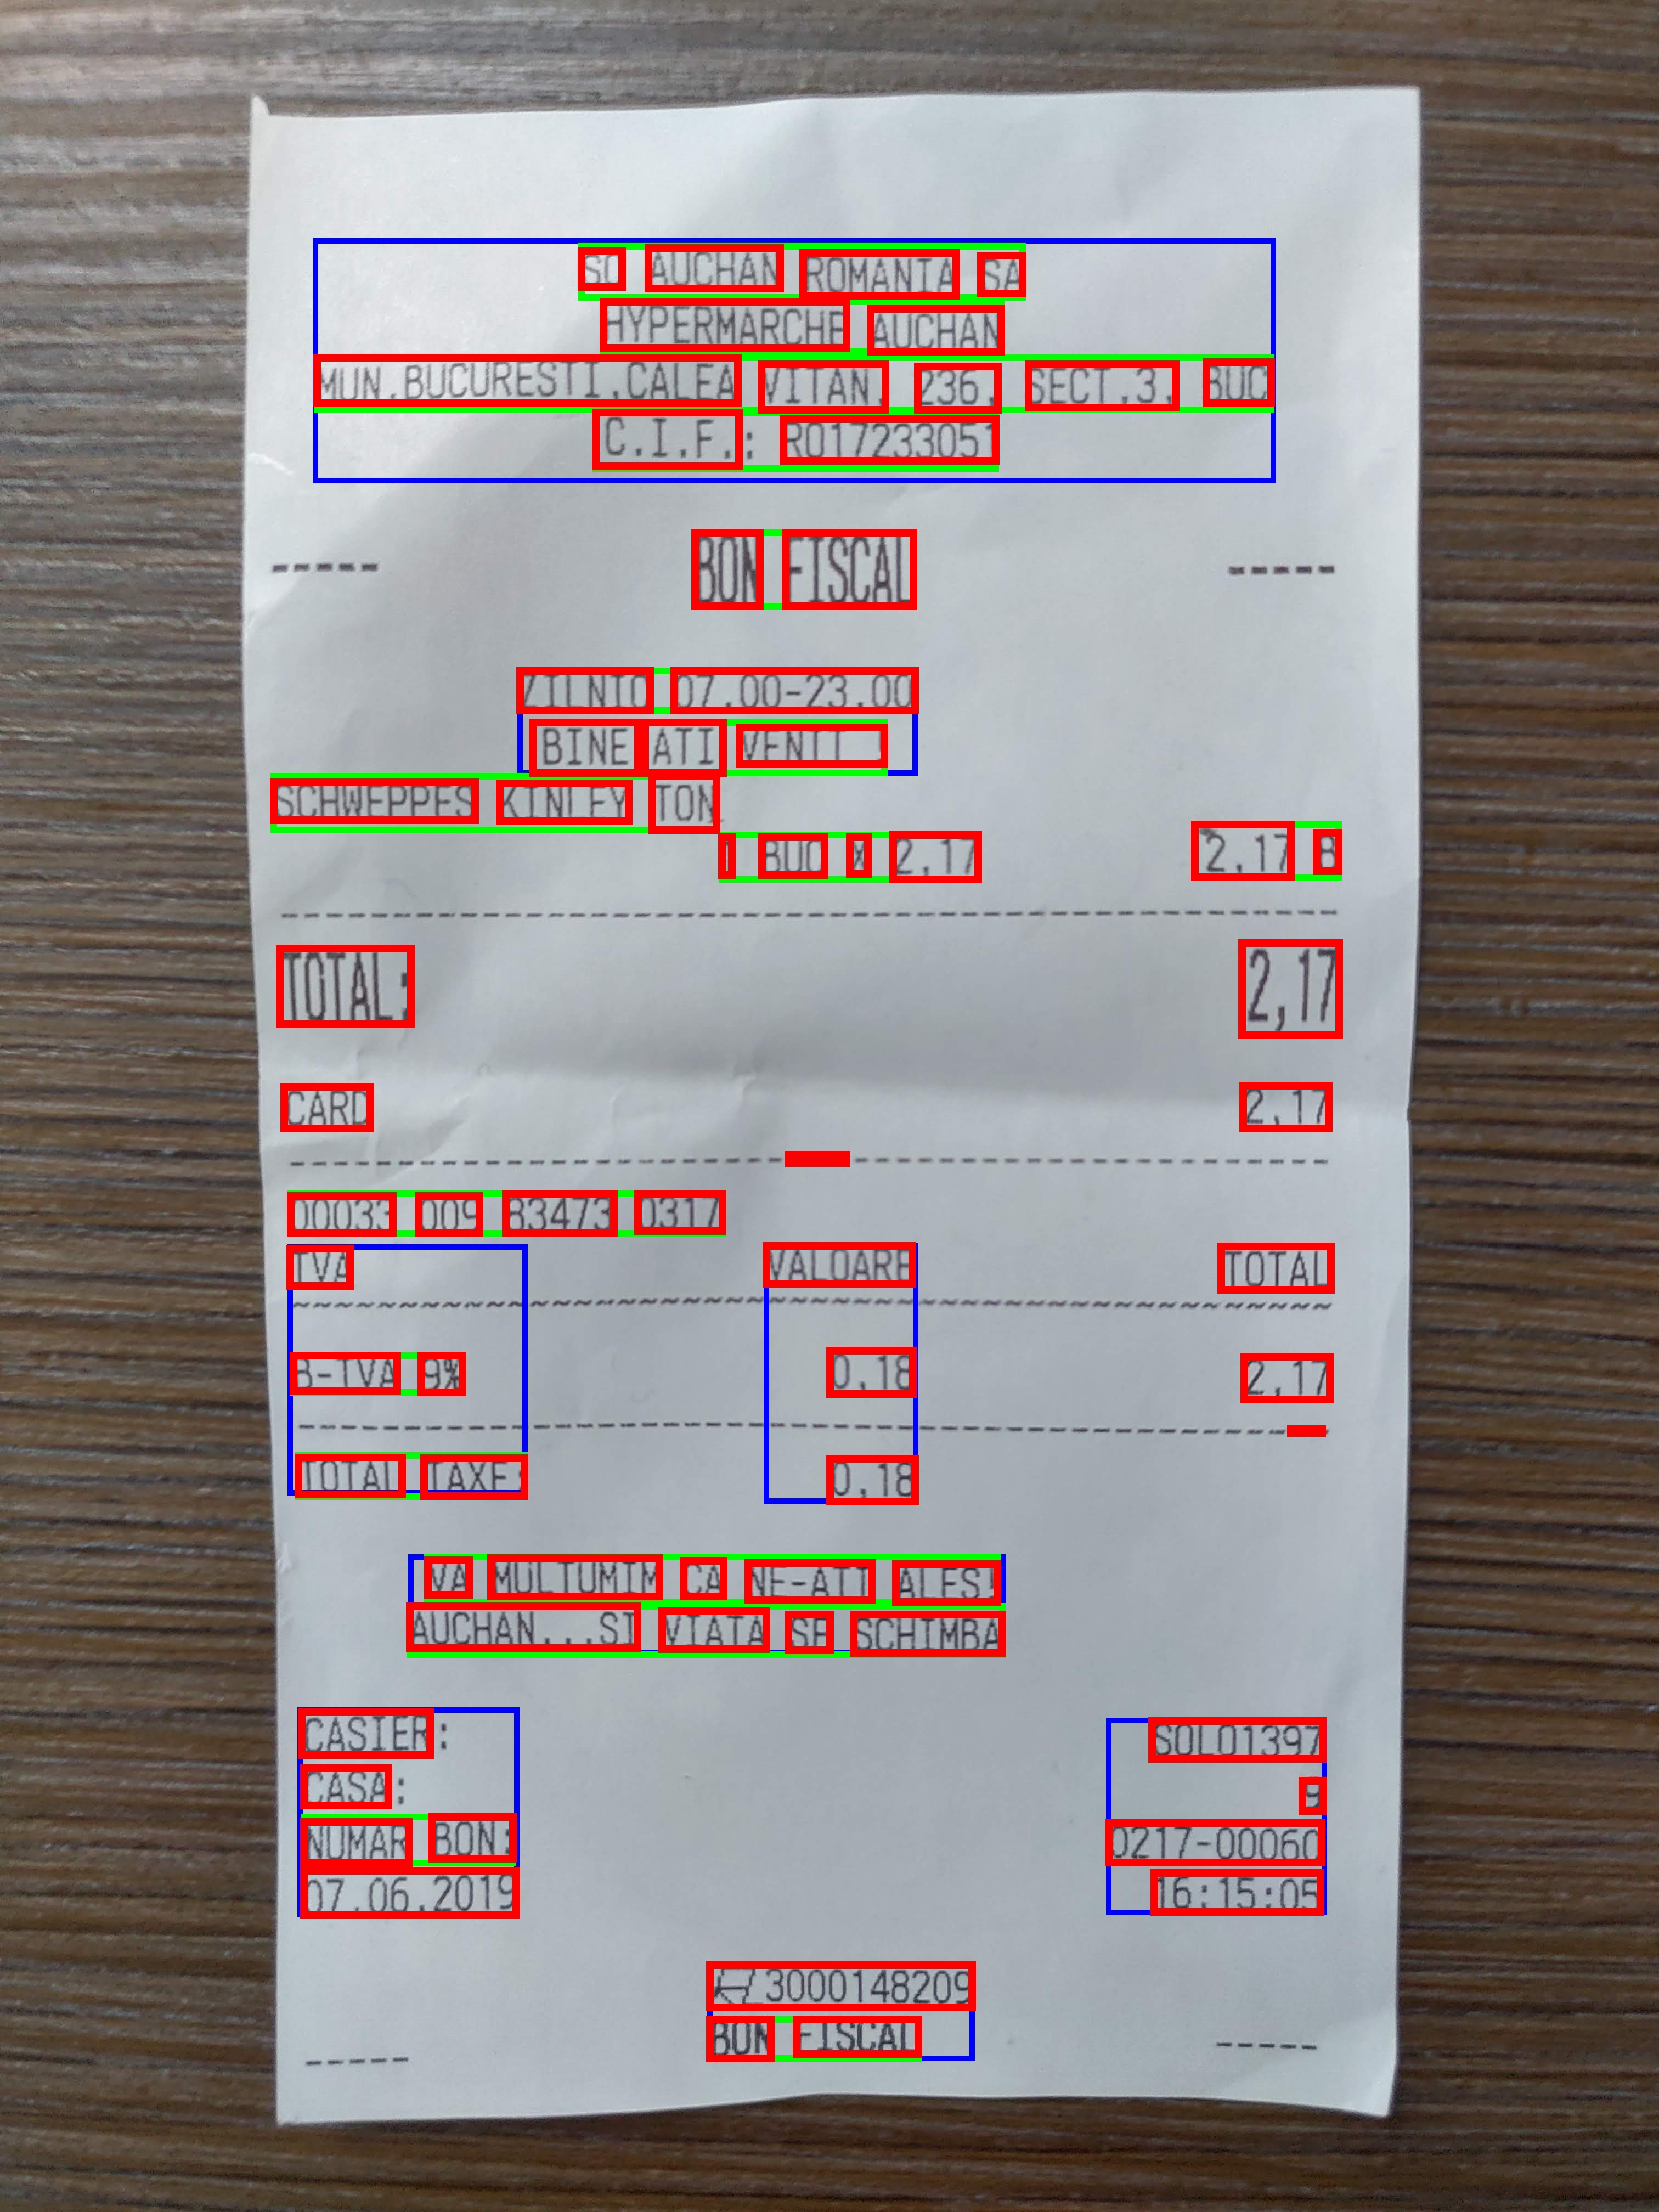
\includegraphics[width=5.5cm]{fibBlocks.jpg}
    \caption{Organizarea rezultatului OCR}
    \label{fig:ocrOutputBoxes}
  \end{subfigure}
  \begin{subfigure}{0.49\textwidth}
    \centering
    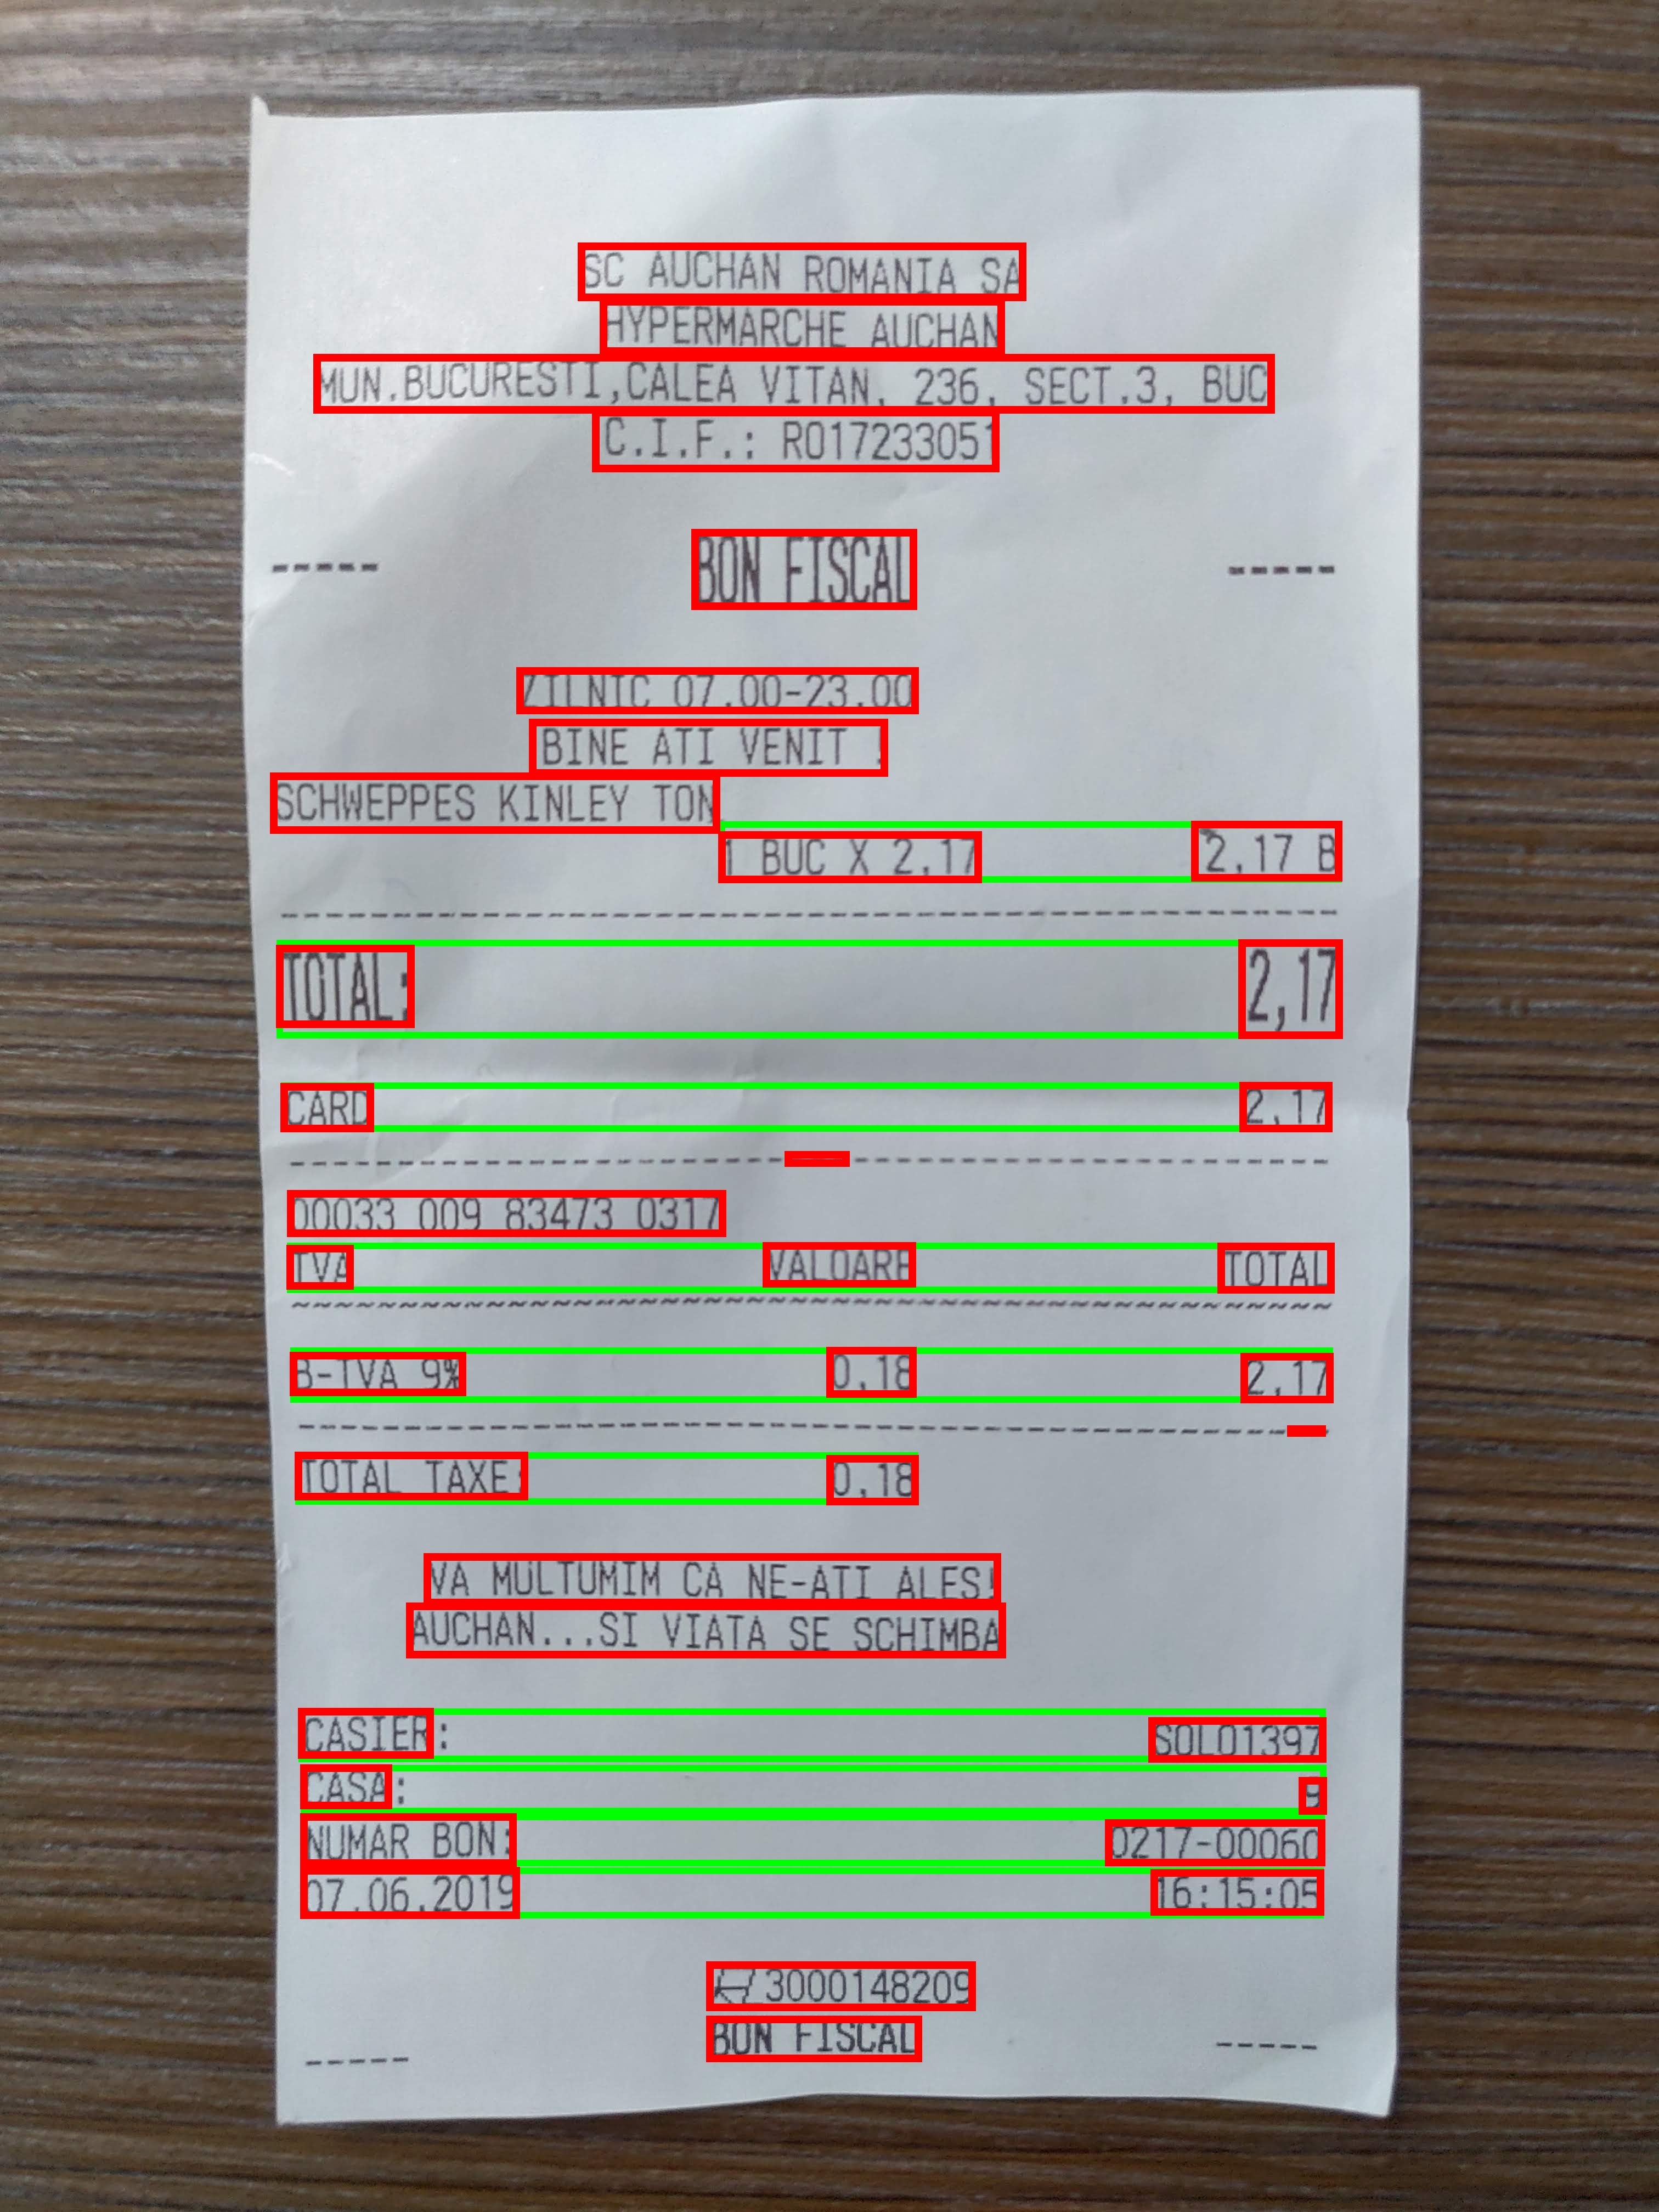
\includegraphics[width=5.5cm]{myBlocks.jpg}
    \caption{Organizarea elementelor OCR dorită}
    \label{fig:desiredBoxes}
  \end{subfigure}
  \caption{Procesul de organizare a rezultatului OCR}
  \label{fig:ocrProcessing}
\end{figure}

Având textul din imagine organizat în grupuri de cuvinte apropiate (vechile linii returnate de \emph{Firebase Vision}) și linii raportate la întreaga imagine, ordonate de sus în jos, informațiile relevante sunt extrase după următoarele reguli:

\begin{itemize}
  \item
  \textbf{Numele comerciantului}:
  \begin{enumerate}
      \item
      Extrage prima linie. Dacă aceasta este formată dintr-o singură literă, continuă extragerea. Această regulă este motivată de faptul că multe bonuri pot conține la început un logo ce poate fi confundat cu o literă.
      \item
      Dacă linia curentă are înălțimea peste media tuturor liniilor, atunci verifică următoarea linie. Dacă și aceasta are înălțimea peste medie și mai puțin de 3 cuvinte, consideră numele comerciantului ca fiind concatenarea celor două linii. În caz contrar, consideră numele comerciantului ca fiind textul liniei curente.
  \end{enumerate}
  \item
  \textbf{Data achiziției}: aplică o serie de expresii regulate pentru a parsa date din întregul text. Dacă sunt găsite mai multe date, alege data cea mai apropiată de data curentă. Dacă nu este găsită nicio dată, consideră data curentă.
  \item
  \textbf{Produse și preț total}: Acestea sunt procesate parcurgând liniile de sus în jos și alcătuind o listă obiecte de tip cheie-valoare. Cheile sunt nume de produse sau cuvinte cheie care să marcheze prețul total, iar valorile sunt prețuri, numere fracționare. Produsele și prețurile aferente sunt considerate toate obiectele care sunt întâlnite deasupra primului obiect ce marchează totalul.
  \item
  \textbf{Categoria și moneda}: aceste valori sunt citite din setările predefinite și pot fi modificate de utilizator.
\end{itemize}

Implementarea detaliată a algoritmului de extragere a informațiilor este prezentată în Anexa \ref{apx:Apendix3}.


